\providecommand{\main}{..}
\documentclass[\main/main.tex]{subfiles}


\begin{document}


\section{Data}

This study is based on the Survey of Health, Ageing and Retirement in Europe (SHARE), a cross-national panel study started in 2004 and conducted every two years. Currently, the survey collects almost 300,000 interviews administered over 6 waves on more than 120,000 respondents from 27 European countries \footnote{Austria, Belgium, Croatia, Czech Republic, Denmark, Estonia, France, Germany,
Greece, Hungary, Ireland, Italy, Luxembourg, the Netherlands, Poland, Portugal, Slovenia,
Spain (including the region of Girona), Sweden, and Switzerland.} and Israele \citep{Bergmann2017}.\\
The SHARE survey is supervised by Prof. Axel Borsch-Supan.\\


SHARE is carried out in an effort to provide high quality data for researchers who want to focus on European population ageing. This is done by asking questions about health, socioeconomic status, social and family networks. The target population is composed by individuals aged 50 and older and their partners.\\ 

SHARE also offers a unified dataset, \textit{easySHARE}, which stores in a single file most of the information collected across the six waves the survey. In \textit{easySHARE}, data are presented in long format and the information collected at couple or household-level is transferred to the individual level. Moreover, the main variables are already coded and do not need extra preparations.
Clearly, for memory consumption issues, only a subset of the many variables of SHARE is included in  the \textit{easySHARE} version. For instance, mortality records are kept in the separate \textit{allwaves\textunderscore cv\textunderscore r}  module.


\section{Data setup}
For the purpose of this analysis, we downloaded both \textit{easySHARE} (Release 6.1.1) and the \textit{All Waves Coverscreen} (Release 6.1.1) from the SHARE Research Data Center as published by June 19th, 2018.\\

The \textit{allwaves\textunderscore cv\textunderscore r} module was then merged to the \textit{easySHARE} dataset.
Out of the 28 countries surveyed in SHARE, we selected only the nine European countries that participated to interview waves 1,2,4,5,6, namely Austria, Belgium, Denmark, France, Germany, Italy, Spain, Sweden, and Switzerland.\\
On the one hand, this means that we are excluding a large part of the dataset but, on the other hand, we have more data points for the selected countries which is likely to increase the precision of our estimates.\\


All records collected in wave 3 of the survey are excluded. This is done because the third wave of SHARE, \textit{SHARE LIFE}, collects very different information compared to other waves: it focuses on people's life histories and, for instance, it does not include information on income. Given the purpose of this investigation, it was therefore impossible to make use of this data.

\subsection{Data cleaning and features generation}

We adopt the approach to drop any observation that contained missing values or inconsistent information with respect to the variables of interest.
The steps taken in each case are briefly outlined below.

\subsubsection{Age}
First of all, we dropped any individual whose age at interview was not reported. Then, we excluded all individuals aged below 50 years old or above 90.
Indeed, even though \textit{easySHARE} specifically targets old population,  the dataset  also  contains  information on  younger  individuals,  i.e.   partners  of  eligible  individuals  aged  50  or  older,  who  are interviewed regardless of their age. Since this population is not the main target of the study and fewer data on this age interval is collected, we decided to excluded it. 
\begin{figure}[H] 
    \centering
    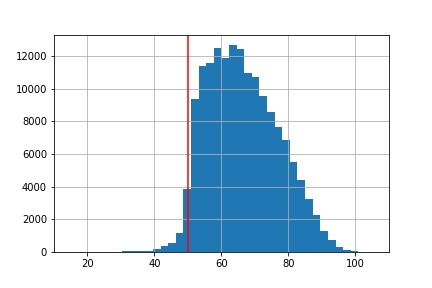
\includegraphics[scale=.5]{images/age_distribution.png}
    \caption{Age distribution of SHARE participants, 9 countries and 5 waves}
\label{fig:age_distribution}
\end{figure}


After we excluded the youngest individuals, we also decided to drop participants aged above 90 years old. Naturally, the number of possible participants decreases at very old ages and the prevalence data collected might be imprecise as well.
\begin{figure}[H] 
    \centering
    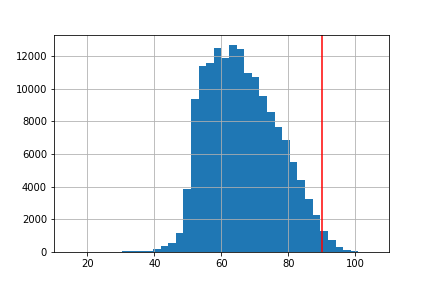
\includegraphics[scale=.5]{images/age_distribution_90.png}
    \caption{Age distribution of SHARE participants, 9 countries and 5 waves}
\label{fig:age_distribution_2}
\end{figure}



\subsubsection{Disability}
From the variable “Activities of Daily Living Index” (ADLA)  of \textit{easySHARE} , we created a  dummy variable representing disability.  In particular,  the variable "Disabled" took value 1 if a respondent reported a functional limitation in at least one of the following tasks: 
\begin{enumerate}
\item dressing
\item bathing or showering
\item eating and cutting up food
\item walking across a room
\item getting in or out of bed.
\end{enumerate}

Respondents who did not report any limitations were considered to be in a healthy status without disability. We dropped all individuals with missing value for adla.

\subsubsection{Income}

In \textit{easySHARE}, the variable \lq\lq $income-pct-w*$'' refers to the net household income. This is computed as the sum of individual imputed income for all components of the household \citep{Adeline2016SomeIncomeb}. 
As reported in \cite{Gruber2014GeneratingProgramming}, the income variable in \textit{easySHARE} is generated in two steps: firstly, country-specific income percentiles are created and, secondly, they are pooled together in a unique income percentile variable.\\

This implies that individuals from different countries might have very different income, in terms of net amount, even thought they have been categorised in the same income percentile. This should be borne in mind when outlining the research question.
However, this paper focuses on computing longevity by income group and country. Therefore, we can use this variable without many concerns as we will be looking at a comparison across individuals within a given country. In other words, we are interested in the distribution of income rather than in the income earned as such.\\

Operationally, we created a variable \lq\lq income'' reporting the individual's income at the time of interview and we eliminated all other variables referring to the net income in previous or subsequent interviews. The logic behind this is that we are interested in the income percentile of the respondent when reporting a disability and we are neglecting the evolution of her income over time. Finally, with respect to the subset of 9 countries we have selected, we find no missing values for the variable \lq\lq $income-pct-w*$''.

\texcolor{red}{check}\\

\subsubsection{Immigrants}
Given that the output of the analysis will be a cross-country comparison of healthy longevity, we worry about a possible "Healthy Immigrant Effect" (HIE) . This phenomenon has been documented in the literature - see, for instance \cite{Deri2004UnderstandingCanada, Kennedy2006TheCountries} - as the fact that, upon  arrival, migrants are typically healthier than the locally-born inhabitants. This might be due to a process of self-selection into migration that leads, ceteribus paribus, healthier persons to migrate more than their unhealthier local counterparts. Nevertheless, as immigrants start to live in the host country, it has been documented that their health status deteriorates, converging to that of the local population or even getting worse.\\
SHARE does not provide any information on the date of migration and taking into account the HIE would complicate the analysis without bringing any significant insights to the research issue. For this reason, we decided to keep only people who were born in the country of interview and drop any missing value or immigrant.


\subsubsection{Deceased age}
As an additional check, we look whether there are some data-entry errors. For instance, we find that some respondents have been reported as dead at an age before the one they have been submitted the interview. This is clearly impossible and hence we drop all these cases.





\end{document}